\documentclass[reqno]{amsart}
\usepackage{amsmath,amssymb,amsthm,amsfonts}
\usepackage{physics}
\usepackage{graphicx}
\usepackage{hyperref}
\usepackage{babel}
\usepackage{qcircuit}
\usepackage{datetime}
\usepackage{ragged2e}
\usepackage{siunitx}
\usepackage{tikz}
\usetikzlibrary{quotes,angles}
\let\oldtocsection=\tocsection

\let\oldtocsubsection=\tocsubsection

\let\oldtocsubsubsection=\tocsubsubsection

\renewcommand{\tocsection}[2]{\hspace{0em}\oldtocsection{#1}{#2}}
\renewcommand{\tocsubsection}[2]{\hspace{1em}\oldtocsubsection{#1}{#2}}
\renewcommand{\tocsubsubsection}[2]{\hspace{2em}\oldtocsubsubsection{#1}{#2}}
\makeatletter
\renewcommand\subsection{\@startsection{subsection}{2}%
  \z@{.5\linespacing\@plus.7\linespacing}{-.5em}%
  {\normalfont\scshape}}
\makeatother

\DeclareMathOperator{\lcm}{lcm}
\newdateformat{monthyeardate}{%
  \monthname[\THEMONTH] \THEYEAR}
\numberwithin{equation}{section}
\numberwithin{figure}{section}

\title{Quantum Computing}
\author[Elliott Ashby]{Elliott Ashby \\ Physics and Astronomy \\ University of Southampton}
\date{\monthyeardate\today}
% ----------------------------------------------------------------

\begin{document}
\begin{abstract}
    Placeholder for abstract.
\end{abstract}
\maketitle
\tableofcontents
\newpage
\section{Introduction}
\begin{justify}
Animals gain advantages in many ways, one of which is the exploitation of properties of the physical world. This has come to culmination in humans; in 1941 we saw the creation of the first programmable computer, the Z3, by Konrad Zuse, and in the following decades we have continually perfected this technology. The modern computer that we use today is, at its fundamental principals, identical to the Z3, performing binary operations on "bits" (a 1 or a 0) of data in order to encode useful computational results. \\

The Z3 used electromagnetic relays (600 in the arithmetic unit, 1,400 to store 64 words) and was close in size to the Stibitz BTL Model 1 or a large, floor-to-ceiling bookshelf. \cite{KonradZuseObituary} In the decades following the Z3, the space required to store and operate computer memory has decreased significantly, and as stated by Moore in 1965, "The complexity for minimum component costs has increased at a rate of roughly a factor of two per year." \cite{Moore1965} This has largely held true, thanks to increasingly smaller and smaller manufacturing processes. \\

As of 2022 the smallest transistors are of the order of 3nm, \cite{Samsung_2022} but when we shrink further down to 2nm or beyond, we begin to approach the size of the atom; at this scale, quantum effects are more pronounced and the transistor can leak current due to gate direct tunnelling. \cite{2nmGateOxide} These effects limit the effectiveness of classical computers at this scale, and so we must look to new technologies to push the boundaries of computation.
\end{justify}

\section{An Overview of Key Concepts}
\subsection{A Brief History of Quantum Computing}
\begin{justify}
During the majority of the 20th century up until the early 1980s the fields of quantum mechanics and computer science were, for the most part, separate areas of study despite some crossover such as the application of the laser. But in 1980, Paul Benioff proposed a quantum mechanical model of the computer and computation process \cite{Benioff1980} and additionally, in the same year, Yuri Manin proposed a similar model. \cite{Manin1980} In the following years, Richard Feynman wrote a paper suggesting that the use of quantum phenomena to perform computations could be more efficient for computer physics simulations than classical computers. \cite{Feynman1982} \\
Just 2 years following this, in 1984, Charles Bennett and Gilles Brassard continued to merge quantum mechanics and computer science by introducing quantum cryptography \cite{BennettBrassard1984} showing that a quantum key distribution can be used to secure communications. \\

Following the proposal of the quantum model of computation, quantum algorithms began to be developed, including Deutsch's algorithm in 1985, \cite{Deutsch1985} the Bernstein-Vazirani algorithm in 1993, \cite{BernsteinVazirani1993} and Simon's algorithm in 1994. \cite{Simon1994} Building on these papers, Peter Shor published his work on prime factorization quantum algorithms which had real world application breaking the RSA and Diffie-Hellman encryption algorithms. \cite{Shor1994} Just 2 years later in 1996, Lov Grover published his algorithm for database search \cite{Grover1996} and in the same year Seth Lloyd finally proved Feynman's conjecture that he proposed in 1982 that quantum computers can be programmed to simulate any local quantum system. \cite{Lloyd1996} \\

The first quantum computer to be built was in 1998; Isaac Chuang and Neil Gershenfeld along with Mark Kubinec implemented Grover's search algorithm with a 2-qubit (the quantum equivalent to bits) nuclear magnetic resonance (NMR) quantum computer. \cite{ChuangGershefeldKubinec1998} In the years following, NMR quantum computers would increase in the number of qubits allowing for a 7-qubit quantum computer to run Shor's algorithm in 2001. \cite{Vandersypen2001} \\

Since then, quantum computing has continued to grow, with new technologies and greater numbers of qubits. The most promising of these is the superconducting circuit used as a qubit. Originally proposed in 1999 by Yasunobu Nakamura, Yuri Pashkin and Jaw-Shen Tsai, \cite{NakamuraPashkinTsai1999} and shown to be viable for greater application in 2007 by Jelle Plantenberg, P.C. de Groot, C.J.P.M. Harmans and Hans Mooij by demonstrating the controlled-NOT gate, \cite{PlantenbergGrootHarmansMooij2007} superconducting qubits have become the focus of many large companies such as IBM and Google. \\

As of 2024, the quantum computer with the most number of qubits is actually not a superconducting quantum computer, but an atomic array quantum computer built by Atom Computing in 2023 \cite{Atom2023, Atom2024} with a reported 1,180 qubits. However, since atomic array quantum computers are much newer than superconducting quantum computers, they have less general support for quantum algorithms; the largest superconducting quantum computer as of 2024 is IBM's Condor with 1121 qubits. \cite{IBM2023, AbuGhanem2024} \\

The field of quantum computing is still in it's infancy, but with promising results and continued growth, it is likely that quantum computers will become more relevant in the coming years.
\end{justify}

\subsection{Limitations of Classical Computers and the Need for Quantum Computing}
\subsubsection{Public-key Cryptography and Factorization of Big Numbers}
\begin{justify}
In 1976, Whitfield Diffie and Martin Hellman published their paper on new directions in cryptography, \cite{DiffieHellman1976} introducing to the general public the concept of public-key cryptography; a method of encryption that uses a pair of keys, public and private, to encrypt and decrypt messages. With the public key, one can encrypt a message that only the private key can decrypt. 2 years later in 1978, Ron Rivest, Adi Shamir and Leonard Adleman published their paper on the "RSA" algorithm, named after their initials, that provides a method for generation of the keys. \cite{RSA1978}\\

The problem of breaking the RSA algorithm is one of finding the prime factors of a large integer. This is difficult to solve for classical computers; the best known algorithm, the general number field sieve (GNFS) \cite{Briggs1998} runs in sub-exponential time, with a time complexity of:
    \begin{equation*}
        O\left(\exp\left[\left(\frac{64}{9}\right)^{1/3}(\log n)^{1/3}(\log \log n)^{2/3}\right]\right) 
    \end{equation*}
    where $n$ is the number to be factorized. If we were to use an $n$ of $2^{2048}$, we would yield a number of operations roughly $\num{1.53e35}$. On a 5GHz CPU on a single thread, this would take $\num{9.72e17}$ years, a long enough time that the RSA algorithm would be considered secure. \\

    However in 1994, Peter Shor published his quantum algorithm for prime factorization \cite{Shor1994} now known as Shor's Algorithm. Shor suggests that a quantum computer could be able to factorize a number in polynomial time $O(\log n)$. The fastest current implementation is of $O((\log n)^{2}(\log \log n))$ \cite{Beckman1996, HarveyHoeeven2021} yielding a number of operations $\num{1.46e7}$. This is a significant speed up over the GNFS and implies that the RSA algorithm is no longer secure. Among security experts, security through obscurity is not considered a valid form of security, \cite{ScarfoneJansenTracy2008} and as such, the need for further research into quantum computing and quantum-resistant cryptography is clear. Shor's Algorithm is discussed further in section \ref{sec:ShorsAlgorithm}.
\end{justify}
\subsubsection{Brute-force Search}
\begin{justify}
Brute-force search is a method of problem solving that involves systematically generating and testing all possible solutions to a problem. That is to say, brute-force search find the single item that satisfies some condition in a unsorted database of $n$ items. Once a single item has been examined, its ability to satisfy the condition can be determined in one step and as such, the most efficient classical algorithms may only determine the correct item in $O(n)$ time, averaging $n/2$ operations. \\

In 1996, Lov Grover published his quantum algorithm for database search \cite{Grover1996} now known as Grover's Algorithm. Grover's Algorithm is able to find this single item in only $O(\sqrt{n})$ steps, and although not a polynomial time speed up, it is still a significant speed up over classical algorithms. Grover's Algorithm is possible since, quantum mechanical systems can be in a superposition of states and simultaneously evaluate the conditions for multiple items in the database. \\

A year later in 1997, Grover's Algorithm was shown to be asymptotically optimal by Charles Bennett, Ethan Bernstein, Gilles Brassard and Umesh Vazirani. \cite{BennettBernsteinBrassardVazirani1997} An algorithm is said to be asymptotically optimal if it, for large inputs, performs at worst a constant factor worse than the best possible algorithm.  Grover's Algorithm is discussed further in section \ref{sec:GroversAlgorithm}.
\end{justify}
\subsubsection{Simulation of Quantum Systems}
\begin{justify}
REDO--- \\
Can physics be simulated on a classical computer? In 1982, Richard Feynman states that it is certainly not possible to simulate quantum systems on a classical computer without infinite time. \cite{Feynman1982} \\

If we wish to simulate a single particle, $\psi$ as a function of $x$ and $t$, it's probability density can be determined classically using numerical methods. \cite{Schroedinger1926} However, if we wish to simulate $n$ particles, the new state of the system is given by some function $\Psi(x_{1}, x_{2}, \ldots, x_{n}, t)$. Describing all of these states would require a $k$-digit number for every configuration of the system, for every arrangement of the $n$ values of $x$. Then, if there are $N$ points in space and each point in space has it's own information such as electric fields, $n$ is of order $N$, so there would be $N^N$ configurations. Since there are too many variables, it cannot be simulated with a classical computer; there are more variables than estimated atoms in the universe! Computing this classically would require to discretize $x$ and $t$ to make any results exact. To do this requires the discarding of terms that are too small, for example if we choose to only take $k$ digits of precision, we must discard probabilities that are less than $2^{-k}$. This is not a problem for a small number of particles, but as the number of particles increases to $n$, the more terms we discard, no matter their validity. \\

Feynman presents that discretizing presents some problems, for example taking the electric field at some point below a certain amount, would in turn suggest that it is not there at all. This is not the case, we know it to be quantized. By discretizing, we are not simulating the correct equations. \\

This leaves only one option, to simulate quantum systems on a quantum computer. Feynman's conjecture was backed up by Seth Lloyd later in 1996 \cite{Lloyd1996} stating that a mere 30 or 40 qubits would be enough to simulate a quantum simulations of multidimensional fermionic systems like the Hubbard model that prove resistant to conventional computers. \\
---
\end{justify}
\subsection{Quantum Bits and Superposition}
\begin{justify}
    The bit is the smallest building block of information of classical information. Similarly, the qunatum bit or qubit is the equivalent for quantum information theory. \cite{Aaronson2013} While the qubit can be represented by physical systems such as photons, electrons or atoms, for now we will consider the qubit as a abstract concept. \\

    While a classical bit has a state of either 0 or 1, qubits similarly have a state of $\ket{0}$ or $\ket{1}$ which correspond to the classical states respectively. There is one key difference however, instead of being exclusively in one state or the other, a qubit can also be in a \textit{linear combination} of states also known as a \textit{superposition}. That is to say, a qubit can be represented as:
    \begin{equation}
        \ket{\psi} = \alpha\ket{0} + \beta\ket{1} \label{eq:qubit}
    \end{equation}
where $\alpha$ and $\beta$ are complex numbers and $|\alpha|^{2} + |\beta|^{2} = 1$. These states however, are not observable, to retrieve information from a qubit, it must be measured. Doing so we get either 0, with a probability of $|\alpha|^{2}$, or 1, with a probability of $|\beta|^{2}$. An example of this could be for a qubit to be in the following states:
    \begin{eqnarray}
        \ket{+} &=& \frac{1}{\sqrt{2}}\ket{0} + \frac{1}{\sqrt{2}}\ket{1} \\
        \ket{-} &=& \frac{1}{\sqrt{2}}\ket{0} - \frac{1}{\sqrt{2}}\ket{1}
    \end{eqnarray}
which we have denoted as $\ket{+}$ and $\ket{-}$.

If we wish to, we can also represent a single qubit using a \textit{Bloch sphere} \cite{FeynmanRichardVernon1957}; a sphere with radius 1 and the poles representing the 2 states $\ket{0}$ and $\ket{1}$. We can rewrite Equation (\ref{eq:qubit}) as:
    \begin{equation}
        \ket{\psi} = \cos\left(\frac{\theta}{2}\right)\ket{0} + e^{i\varphi}\sin\left(\frac{\theta}{2}\right)\ket{1}
    \end{equation}
where $\theta$ and $\phi$ are the angles of the Bloch sphere shown in Figure \ref{fig:BlochSphere}. Operations on single qubits can be represented as rotations on the Bloch sphere, which is a useful way to visualize quantum operations. \\
    \begin{figure}[h]
        \centering
        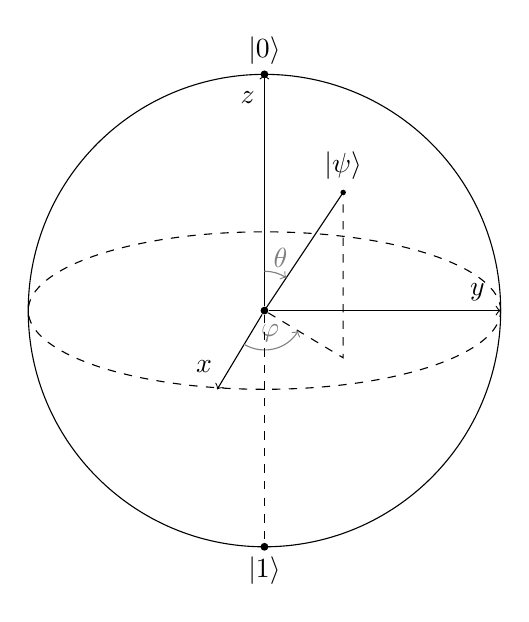
\begin{tikzpicture}

              % Define radius
              \def\r{3}

              % Bloch vector
              \draw (0, 0) node[circle, fill, inner sep=1] (orig) {} -- (\r/3, \r/2) node[circle, fill, inner sep=0.7, label=above:$\ket{\psi}$] (phi) {};
              \draw[dashed] (orig) -- (\r/3, -\r/5) node (phinode) {} -- (phi);

              % Sphere
              \draw (orig) circle (\r);
              \draw[dashed] (orig) ellipse (\r{} and \r/3);

              % Axes
              \draw[->] (orig) -- ++(-\r/5, -\r/3) node[pos=0.9, above left] (x1) {$x$};
              \draw[->] (orig) -- ++(\r, 0) node[pos=0.9, above] (x2) {$y$};
              \draw[->] (orig) -- ++(0, \r) node[pos=0.9, left] (x3) {$z$};

              % Angles
              % \pic["$\phi$", draw=gray, text=gray, ->] {angle = x1--orig--phi};
              % \pic["$\theta$", draw=gray, text=gray, <-, angle eccentricity=1.4] {angle = a--orig--x3};
          	  \path (orig) ++(-\r/10, -\r/6) coordinate (phi_start); % Start point for phi
              \pic [draw=gray, text=gray, ->, "$\varphi$"] {angle = phi_start--orig--phinode};
              \path (orig) ++(0, \r/2) coordinate (theta_start); % Start point for theta
              \pic [draw=gray, text=gray, <-, "$\theta$", angle eccentricity=1.4] {angle = phi--orig--theta_start};

              % Kets at poles with nodes
              \node[circle, fill, inner sep=1] at (0, \r) {}; % North pole node
              \node[above] at (0, \r) {$|0\rangle$};          % Label for north pole
              \node[circle, fill, inner sep=1] at (0, -\r) {}; % South pole node
              \node[below] at (0, -\r) {$|1\rangle$};
              \draw[dashed] (orig) -- (0, -\r); % Dashed line orig and south pole

        \end{tikzpicture}
        \caption{The Bloch Sphere}
        \label{fig:BlochSphere}
    \end{figure}

    Despite the fact that a single qubit has an infinite number of possible states (all possible values of $\alpha$ and $\beta$), we cannot use a qubit to store an infinite amount of data. This is because in order to extract any information from a qubit it must be measured; measurement results in a collapse from its superposition of $\ket{0}$ and $\ket{1}$ to either 0 or 1. This means that any further measurements are guaranteed to yield the same result. For example, if measurement of $\ket{-}$ gives 1, then any additional measurements must also give 1. \\
\end{justify}
\subsection{Quantum Superposition of Multiple Qubits and Entanglement}
\begin{justify}
    Just as a single qubit can be in a superposition of states, multiple qubits can be in a superposition of states. For example, a 2-qubit system can be in a superposition of 4 states:
    \begin{equation}
        \ket{\psi} = \alpha_{00}\ket{00} + \alpha_{01}\ket{01} + \alpha_{10}\ket{10} + \alpha_{11}\ket{11}
    \end{equation}
    where $\alpha_{00}$, $\alpha_{01}$, $\alpha_{10}$ and $\alpha_{11}$ are complex numbers and $|\alpha_{00}|^{2} + |\alpha_{01}|^{2} + |\alpha_{10}|^{2} + |\alpha_{11}|^{2} = 1$. Similarly to a single qubit, the probability of measuring a state $\ket{xy}$ is $|\alpha_{xy}|^{2}$. However we could potentially only measure one of the two qubits, collapsing that one but not the other. If we measured the first qubit to be 1, then new state of the system would then be:
    \begin{equation}
        \ket{\psi'} = \frac{\alpha_{10}\ket{00}+\alpha_{01}\ket{01}}{\sqrt{\abs{\alpha_{10}}^{2} + \abs{\alpha_{11}}^{2}}}
    \end{equation}
\subsection{The Thermodynamics of Quantum Computing}
\subsection{Quantum Algorithms and Parallelism}
\subsubsection{Deutsch's Algorithm}
\subsubsection{Bernstein-Vazirani Algorithm}
\subsubsection{Simon's Algorithm}
\subsubsection{Shor's Algorithm} \label{sec:ShorsAlgorithm}
\begin{justify}
The RSA algorithm uses 3 large positive integers, $e$, $d$ and $n$, where $n$ is the product of 2 large prime numbers, $p$ and $q$, and for all integers $m(0 \leq m < n)$, both $(m^{e})^{d}$ and $m$ have the same remainder when divided by $n$. That is to say:
    \begin{equation}
        (m^{e})^{d} \equiv m \mod n
    \end{equation}
where $n$ and $e$ make up the public key, $d$ is the private key, and $m$ is the message. We can then define the encryption and decryption as follows: 
    \begin{eqnarray}
        c &\equiv& m^{e} \mod n \label{eq:RSAencrpyt} \\
        m &\equiv& c^{d} \mod n
    \end{eqnarray}
where $c$ is the cipher text. \\

The RSA algorithm is said to be secure because breaking it requires recovering $m$ such that Equation (\ref{eq:RSAencrpyt}) is true. To do this requires the factorization of $n$ into its prime factors, hence allowing the calculation of $d$ from $e$ and the prime factors of $n$.
\end{justify}
\subsubsection{Grover's Algorithm} \label{sec:GroversAlgorithm}
\subsection{Quantum Error Correction}
\subsection{Experimental Quantum Computing}

\bibliographystyle{unsrtdin}
\bibliography{citations}
\end{document}
